 \documentclass{article}

%%%%%%% PACKAGES %%%%%%%%
% \usepackage{mathptmx}

\usepackage[utf8]{inputenc}
\usepackage[margin=2cm]{geometry}
\usepackage{blindtext}
\usepackage{tabularx}
% \usepackage{setspace}
\usepackage{graphicx}
\usepackage{notoccite} %citation number ordering
\usepackage{lscape} %landscape table
\usepackage{caption} %add a newline in the table caption

\usepackage[
backend=biber,  %references format (IEEE)
style=ieee,
sorting=none
]{biblatex}
\addbibresource{refs.bib} %rename this to your own bibliography
% \onehalfspace   % 1.5 line spacing

\title{\textbf{ Indian Institute of Information Technology, Allahabad 
}}
\date{\LARGE\textbf{Department of Information Technology}}

\begin{document}

\pagenumbering{roman} % Start roman numbering
\clearpage\maketitle

\thispagestyle{empty}

\begin{center} 
    \begin{figure}[h]
        \centering
        
\includegraphics[width=5cm]{pics/iiitalogo.png}
        %\caption{Your caption here}
        \label{fig:logo}
    \end{figure}
    \vspace{5mm}
    \textbf{Image and Video Processing Course 2021}\\ \vspace{5mm}
    \textbf{Progress Report}\\	\vspace{5mm}
     \textbf{on }\\	\vspace{5mm}
       \textbf{Smart Agro Kit }\\	\vspace{5mm}
         \textbf{as }	\\\vspace{5mm}
         \textbf{part of C1 assessment }\\	\vspace{5mm}
         \textbf{by }\\	\vspace{5mm}
        
     
     \smallskip
    % \vfill
    %  \hfill Submitted. By\\
    %  \hfill Mrityunjaya Tiwari : IIT2019239\\
    %   \hfill Mrityunjaya Tiwari : IIT2019239\\
    %   \hfill Mrityunjaya Tiwari : IIT2019239\\
    %     \hfill Mrityunjaya Tiwari : IIT2019239\\
     

     
     \begin{tabular}{ |p{7cm}|p{7cm}|p{7cm}|  }
\hline
Name& Enrollment Number \\
\hline
Mrityunjaya Tiwari & IIT2019239\\
                    Raunak Singh Rathore  & IIT2019222\\
                     Amanjeet kumar  & IIB2019006\\
                      Jyoti Verma  & IIT2019202\\
                        Noonsavath Sravana Samyukta & IIT2019236\\
                          Raj Chandra & IIT2019200\\
\hline
\end{tabular}
         
         

    
\end{center}
\newpage
\setcounter{page}{1}
\tableofcontents
\newpage


\pagenumbering{arabic} % Start roman numbering

%%% CONTENT HERE %%%%
\section{Abstract}
\large{One of the important and tedious tasks in agricultural practices is detection of disease on crops. It requires a huge amount of time as well as skilled labor. So for detection of diseases on crops we propose a smart and efficient technique which uses image processing and IoT techniques that analyse crops and send alerts with disease names and how to prevent as well to the farmers.}
\section{Introduction}
\large{we know Mostly Farmers live long distance from their field, they have to walk everyday to see the status of the crop and also Farmers owns multiple fields, but are away from each-other,being updated at all time for Farmers about the rainfall status, humidity and climatic conditions priory isn't possible many times This is the reason for many crops failure. As a solution the aim of our project work is to develop a reliable and easy to use system for use by farmers. The major goal of the project is to make farmers update about their crops anytime. What we are gonna do is We'll set a camera in our kit that clicks photos of crops that will take readings continuously through the micro controller and send them to the cloud . We'll train a deep learning model for detection of diseases of crops. If any disease will be detected by our model, then it will send alerts with disease names and how to prevent as well. and also manually farmers can take pictures of crops and then the system will check whether everything in crops is ok or not then will notify farmers about it. }

\section{Literature Survey}
\large{Plant  diseases are  generally  caused  by  infectious agents  such  as  fungi,  bacteria,  and  viruses.  Signs  of plant disease are observable evidence of infection and symptoms are  the  visible  effects  of  these  kinds  of  disease. 
\bigskip

Fungal infections  cause  signs  like  visible spores,  mildew,  or  mold and the basic symptoms are like leaf spot and yellowing. Fungal   diseases are   plant   infections   caused   by fungi.  Fungi  can  be  single  or  multicellular,  but  either  way infect   plants   by   stealing   nutrients   and   breaking   down tissue. \\
 Fungal diseases  are  the  most  common  infection  in plants. \\\\

 Fungi  infections  can  be  recognized  by  symptoms like  spots  on  plant  leaves,  yellowing  of  leaves,  and  birds-eye   spots on   berries.   With   some   fungal   diseases,   the organism itself can actually be viewed on the leaves as a growth and as a mold .
 }

\section{Methodology being used}

The  process of  developing Smart Agro kit  basically involves  four  phase:

\subsection{Image Acquisition :} In  this  phase,  images  of  plant  leaves  are  gathered using  digital  media with desired  resolution  and  size. Smart Agro kit consists of a camera system to capture real time photos of crops at some interval and this camera is connected to a micro controller that will send images to the cloud for disease detection . Users can also upload crop images on the web . 

\subsection{Image Segmentation:} This  phase  aims  at  simplifying  the  representation of  an  image  such  that  it  becomes  more  meaningful  and easier to Analyze. There  are  various  methods  using  which  images can   be   segmented   such   as   k-means  clustering,  Otsu’s algorithm  and  thresholding  etc.   The  k-means  clustering classifies objects or pixels based on a set of features into K number    of    classes.    The    classification is done by minimizing  the  sum  of  squares  of  distances between the objects and their corresponding clusters. 

\subsection{Classification:} This classification  phase  implies  to  determine  if the input image is healthy or diseased. We are training a model to detect crop diseases with different different data sets . We are currently working on model training .

 
\begin{center}
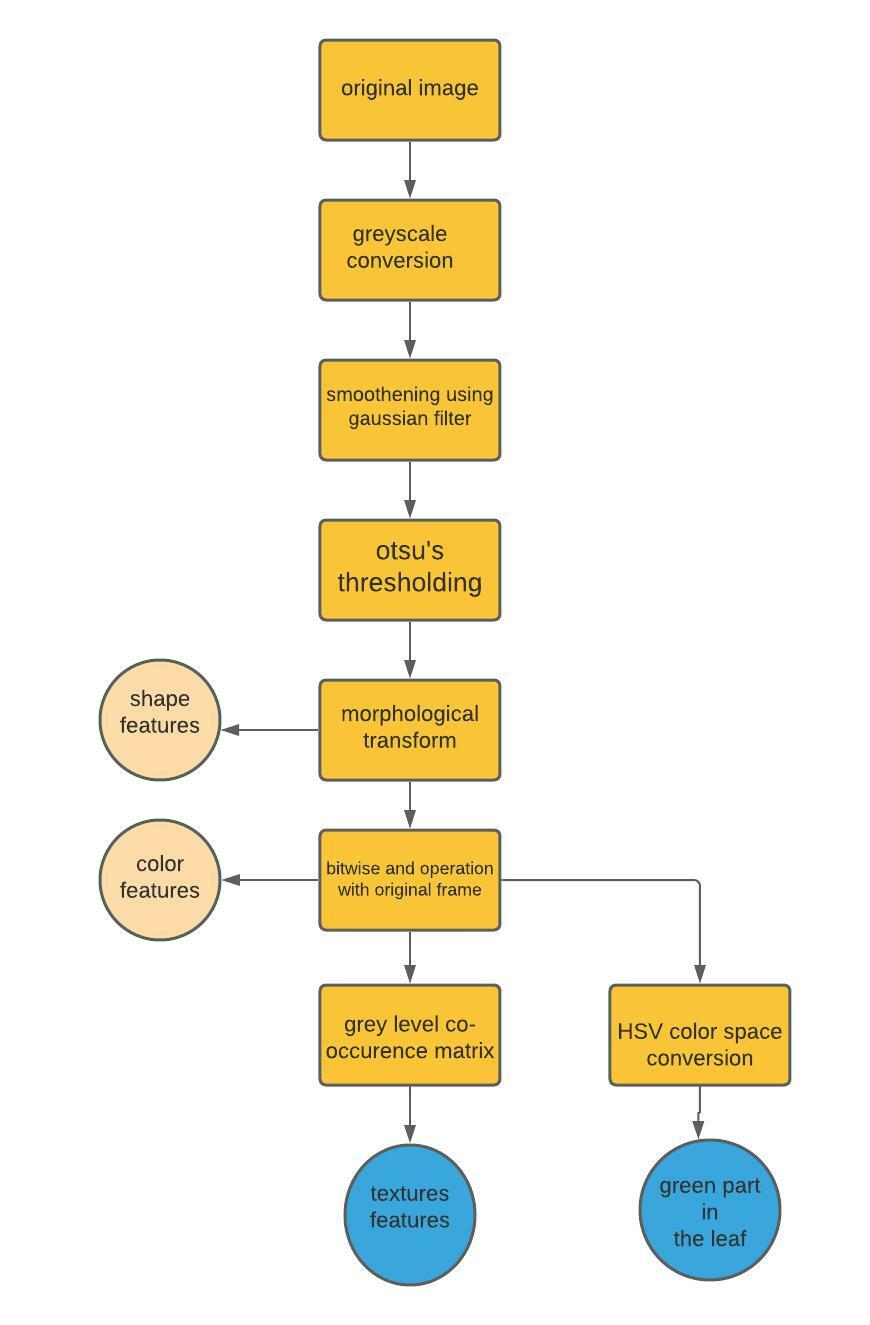
\includegraphics[width=10cm]{pics/class.jpeg}
\end{center}



\subsection{Sending alerts:}  Crop’s images are clicked by camera system and sent by microcontroller to cloud for disease detection.  If there is any disease detected then SMS/mail will be sent out to the farmers with disease names as well as prevention methods of that particular disease . We are using Twilio API for sending text alerts and Mailgun API for sending emails .\\

\begin{center}
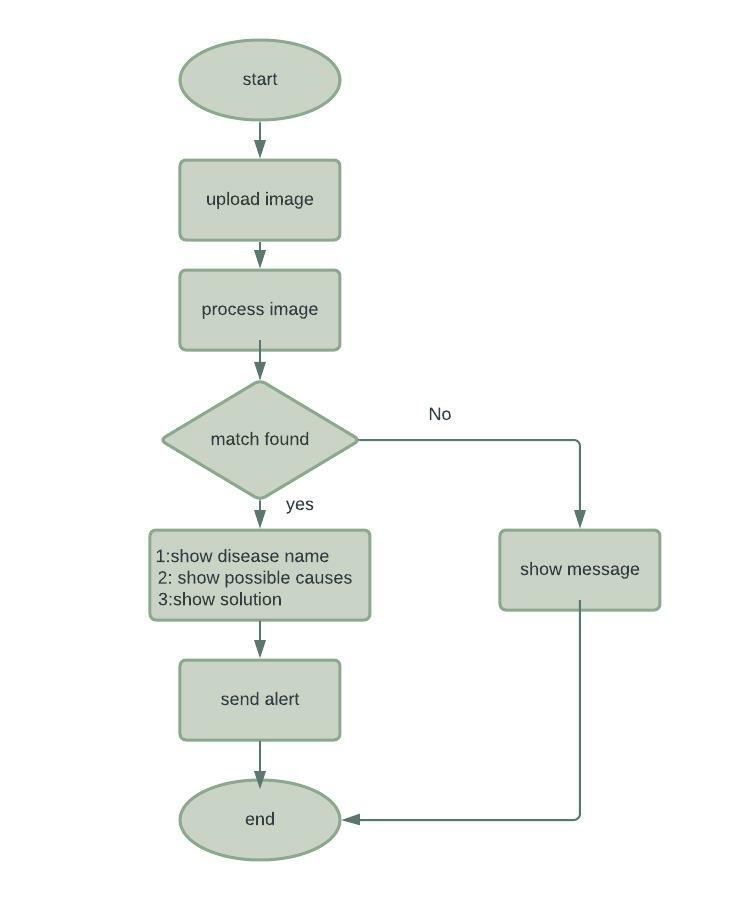
\includegraphics[width=15cm]{pics/drawivp (2).jpeg}
\end{center}

\section{Datasets being used}
\large{For this project we have used a public data set for plant leaf disease detection.}

\bigskip
\textbf{Kaggle Link of datasets:}\\
\large{\url{https://www.kaggle.com/vipoooool/new-plant-diseases-dataset }}

\bigskip
\textbf{Sample images of datasets:}\\\\
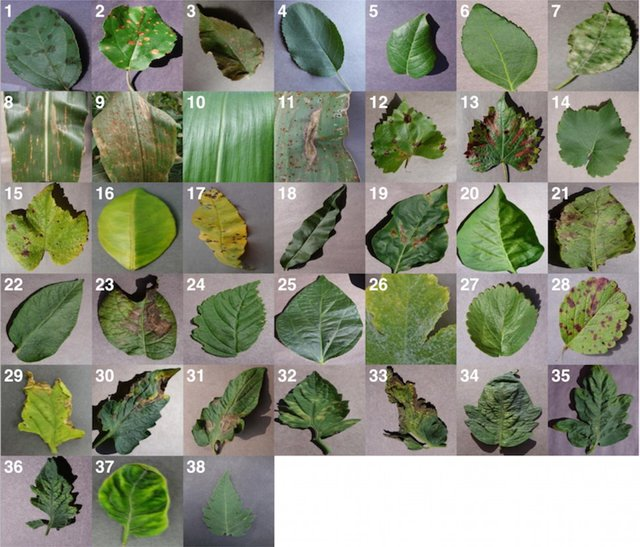
\includegraphics[width=15cm]{pics/dataset.jpeg}

\section{Results and Discussion}
\large{There are two  different  conditions  for  training  and testing.  One  is  under  the  lab  conditions,  which  means  that the  model  is  tested  with  the  images  from  the  same  dataset from  which  it  is  used  for  both  training  and  testing.    The other  condition  is  that  field  condition;  this  means  that  our model has been tested with the images taken from the real world conditions   (land).   Since   the   lighting   conditions   and background  properties  of  the  images  are  totally  different when we take samples from the real field, there is a chance that  our  model  to  produce  a  very  low  accuracy,  when comparing  to  the  accuracy  values  acquired  during  the  lab conditions.\\\\  
So  to overcome  this  impact,  we  had  an  idea  of having a mixed variety of images during           the training phase .

}

\section{Conclusion}
\large{So in the proposed project system, by using image processing and IoT techniques that are capable of monitoring the crops, analysing the disease names and also sending alerts to the farmers. The system consists of both hardware and software parts. Different Argo sensors are used to detect the diseases and take readings continuously through micro controller and send data to the cloud. If readings are not in range of threshold values then the system will send alerts via sms. 
}
\section{Individuals contribution}
\subsection{IIT2019239: Mrityunjaya Tiwari}
\large{My contribution on this project is to connect micro controller with cloud and deploying model on Amazon AWS . I also contributed in documentation and designing the webpages.}

\subsection{IIB2019006: Amanjeet Kumar}
\large{My contribution on this project is to train model for disease detection , linking model with Twillo , Mailgun APIs and contributed in documentation. I also designed the UML diagrams for the project.}

\subsection{IIT2019222: Raunak Singh Rathore}
\large{My contribution on this project is to  train ML model and deploying model on Amazon AWS . I contributed in documentation.I have also contributed in web page designing. }
%
\subsection{IIT2019202: Jyoti Verma}
\large{My contribution on this project is to train model for disease detection , linking model with Bolt clouds APIs and I also contributed in documentation.}


\subsection{IIT2019236: N Samyukta}
\large{My contribution on this project is to find out datasets project development . I also contributed in documentation and designing the webpages.}

\subsection{IIT2019200: Raj Chandra}
\large{My contribution on this project is to develop webpages and I also contributed in documentation.}


\section{References}
\begin{itemize}
  \item \url{https://ieeexplore.ieee.org/document/8697390 }
  \item S. D.M., Akhilesh, S. A. Kumar, R. M.G. and P. C., "Image based Plant Disease Detection in Pomegranate Plant for Bacterial Blight," 2019 International Conference on Communication and Signal 
  \item Identifying two tomato leaf viruses using a support vector machine, in: Information Systems Design and Intelligent Applications : U. Mokhtar, M.A. Ali, A.E. Hassanien, H. Hefny,
  \item Bashish,   D.A.,   Braik,  M.,  Ahmad,  S.B.,  ‘A  Framework  for Detection and Classification of Plant Leaf and Stem Diseases’, International  Conference  on  Signal  and  Image  Processing,  pp. 113-118, 201 

\end{itemize}


 

\end{document}

\newpage
\setstretch{1}  %reduce bibliography line spacing
\printbibliography
\end{document}
